
\section{OpenStack Deployment Tools}

There are many ways how to deploy OpenStack infrastructure which are more or less automated. Some of them require to fill in answer files, some configuration files. Some tools have graphiceal user interface and allow to provision entire hardware infrastructure as some just configure the services on the provisioned servers.

Model je popsanej dokumentem a není to čitelný, automatizace. Není validita modelu. Chyby se debugují na úrovni reality.

\begin{figure}[!h]
\centering
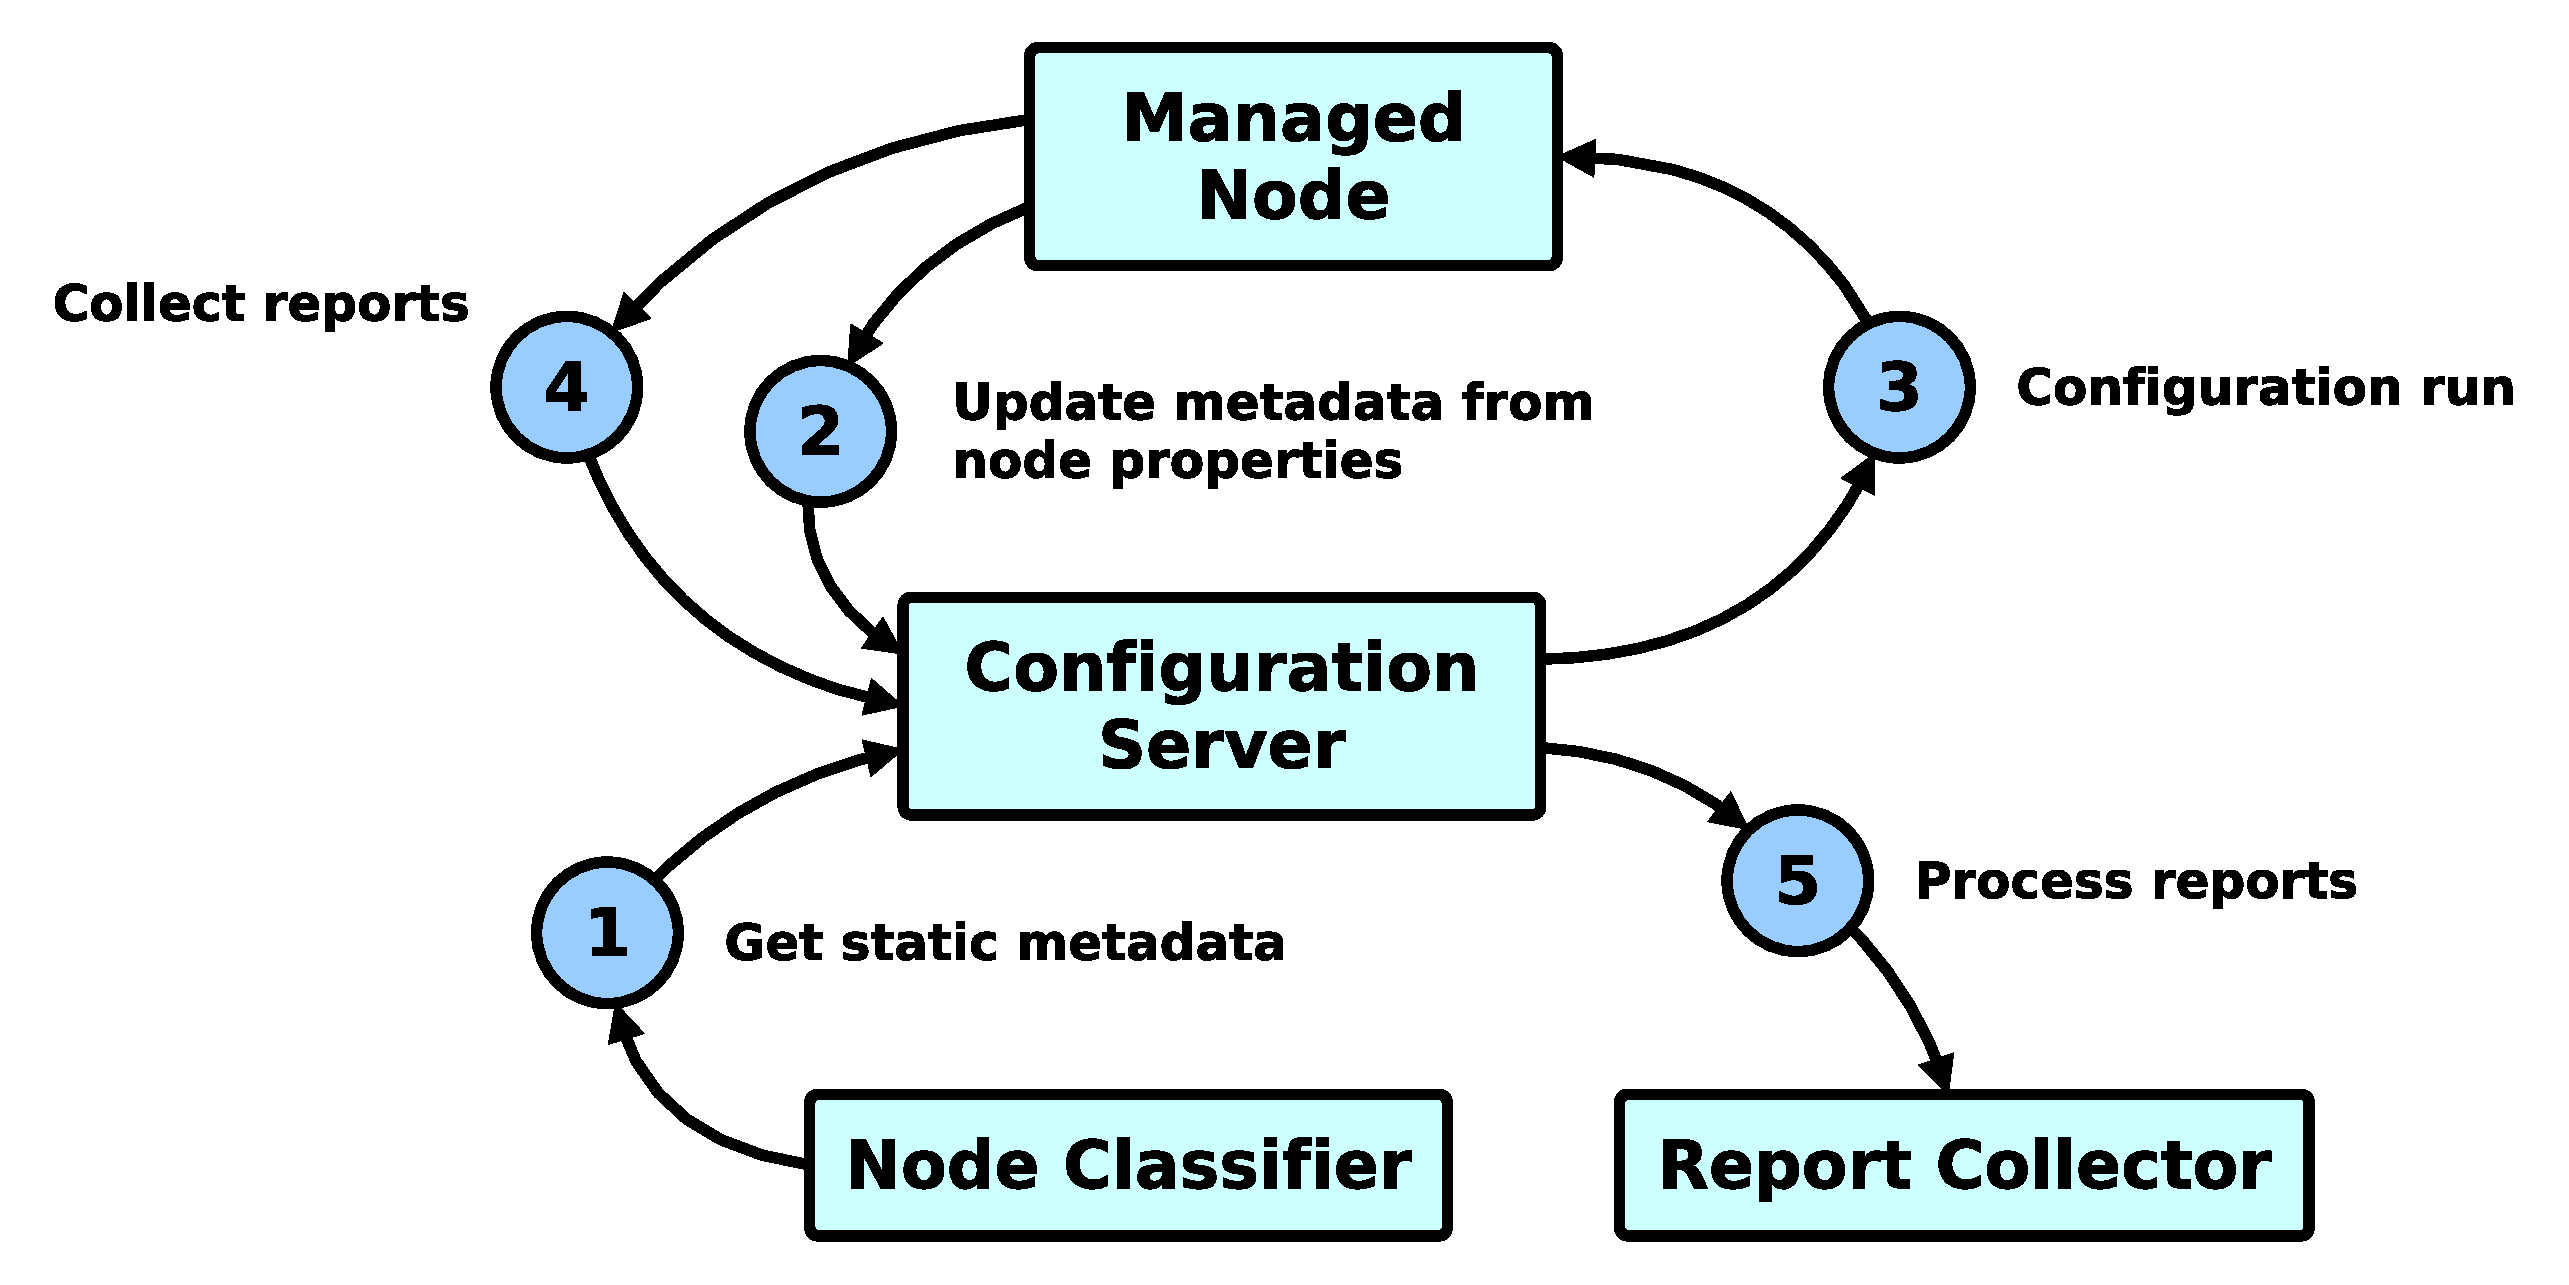
\includegraphics[scale=.15]{img/cm_cycle.eps}
\caption{Configuration Management deployment cycle}
\label{fig:cm}
\end{figure}


\subsection{Development}

For testing and developing OpenStack ...

\subsubsection{PackStack}

\subsubsection{Devstack}

\subsection{Production}

\subsubsection{Fuel}

\subsubsection{Foreman}
